\section{Evaluation}
\subsection{Generated image channel}
The channel suite creates \BenchTrials{} independent source markers using fresh
keys, statements and challenges, then pairs fourteen transformations within each
source. It performs \ChannelObservations{} actual raster decode attempts. Conditions
include clean and 90-degree rotation, an 8\% perspective warp, Gaussian blur at
0.8, 2 and 4 pixels, contrast 0.35, resizing to 50\% and 15\%, JPEG quality 35,
Gaussian pixel noise of standard deviation 25, square occlusions with side lengths
8\% and 25\% of image width, and a neighboring instruction panel. Occlusion
percentages refer to side length, not covered image area. Success requires exact
recovery of the original signed bytes.

\begin{figure*}[t]
\centering
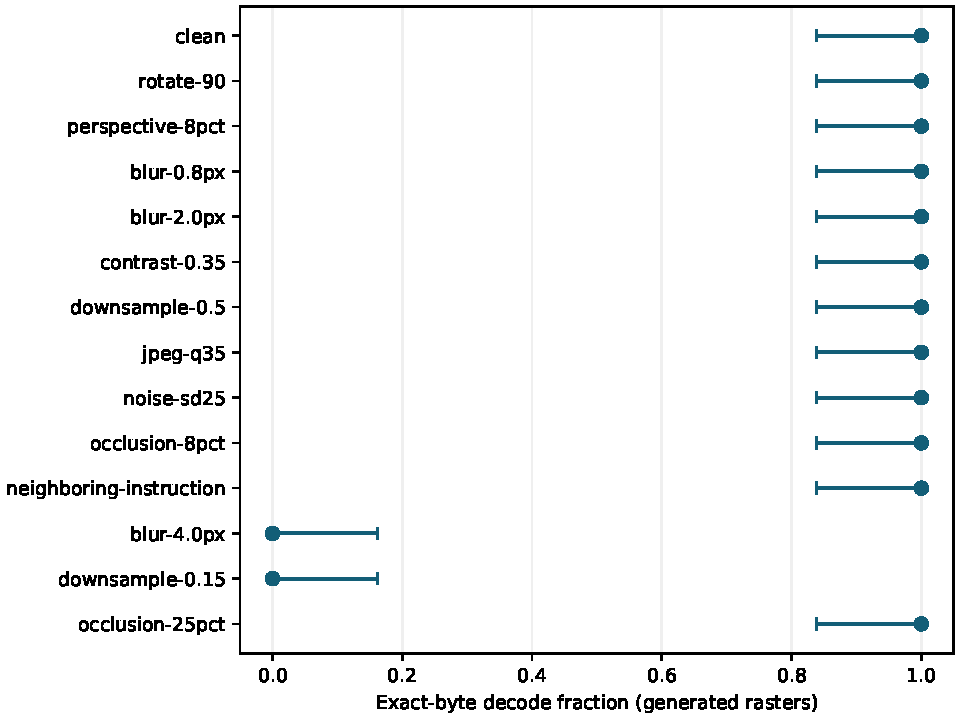
\includegraphics[width=0.85\textwidth]{artifacts/channel.pdf}
\caption{Exact-byte recovery on generated rasters, 20 source images per condition.
Bars are descriptive 95\% Wilson intervals. Conditions share source markers; the
figure is not a camera study or a deployment-security estimate.}
\label{fig:channel}
\end{figure*}

Clean images decoded in \CleanSuccesses{}/\BenchTrials{} trials, with median
\CleanMedian{} ms and p95 \CleanPninetyfive{} ms. Severe 4-pixel blur and 15\%
resizing failed in the recorded suite. The remaining conditions recovered all
recorded markers, without a successful decode yielding different bytes. These
results describe this codec, marker density and generated image family; they do
not generalize to arbitrary cameras, lighting, perspective or materials. A 20/20
condition still has a wide Wilson interval and is not a universal reliability
claim. The neighboring-instruction case demonstrates byte isolation only; no
language model interprets the instruction panel.
\subsection{Policy controls and schedules}
The serial suite repeats every named case \BenchTrials{} times with fresh keys,
challenges and temporary SQLite state. It includes changed principals, actions,
resources, purposes and arguments; altered signatures; unconfigured keys; session
and nonce transplantation; wrong audience; expired challenges and grants; grant
and issuer revocation; unregistered permission; wrong grant scope/modality;
consumed replay; malformed observation profiles; unsupported guarantees and
unaccepted assumptions. Modality-specific cases extend this common taxonomy.

An intentionally weak signature-only ablation ignores scope, freshness and
permission. It isolates why authentication alone is insufficient; its failures
are not evidence against correctly configured existing authorization. An equally
expressive sequential typed-policy control separately checks the same expected
challenge, action, supported guarantees and permission state. It shares
cryptographic and modality validators with the gateway and is not an independent
audit, full IFC implementation or reimplementation of published agent defenses.

The concurrency suite runs \BenchTrials{} trials of eight duplicate attempts
released together; each must produce exactly one receipt. Another
\BenchTrials{} trials hold the write boundary, revoke the grant and then release a
worker's commit. Every such prior-revocation schedule must produce zero receipts.
This is a deliberately selected serialized order, not an exhaustive scheduler
exploration. Tests also check rollback, expiry at the boundary and replay after
restart.

\subsection{Interpretation}
Across \SecurityObservations{} serial case observations
(\SecurityCases{} cases per trial), the gateway produced
\UnauthorizedEffects{} unauthorized new local receipts and
\TypedDisagreements{} disagreements with the typed control. The weak
signature-only check accepted \SignatureFalseAccepts{} observations that violated
the specified policy. Mixed accepted/denied gate processing had median
\GateMedian{} ms and nearest-rank p95 \GatePninetyfive{} ms. These one-host
measurements include SQLite work for accepted requests, but are not a matched
latency comparison with the control or an end-to-end physical delay.

Two limitation cases deliberately accept valid structured responses: transparent
live forwarding when no proximity guarantee is required, and a configured
attester producing a plausible report when sensor truth is not required. These
are modeled traces, not physical relay or compromised-device experiments. Requiring
proximity or consent is separately denied. Denial is not a result demonstrating
those properties. Channel trials and policy cases are distinct suites; the
runnable demos combine channel parsing, signature appraisal and effect insertion.

\subsection{Validity and missing comparisons}
Fresh source markers provide trial variation, but condition order is fixed and
all timing runs share one host. No matched comparison with a static signed-code
codec, authenticated API or physical-factor system is reported. The dataset is
small, synthetic and selected by the implementation authors. We release all
case rows and failures rather than interpreting zero observed policy violations
as a deployment attack probability. A future study needs camera/display trials,
physical relays, held-out scenes, independent review and agent-level disclosure
metrics across every enabled output.

